% ******************************* APPENDICE B - GUIDA AL CODICE ********************************

\chapter{Guida al Codice}
\label{appendice2}

In questa Appendice si descrive il codice utilizzato suddividolo in \verb!package!, la cui repository è disponibile all'indirizzo \href{https://github.com/ProgettoSGN/charlie}{GitHub}.

All'utilizzo pratico, i file qui descritti vengono eseguiti tramite 5 launch file presenti all'interno del package \verb!charlie_pkg! realizzato ad hoc per il robot.

\bigskip

I 5 launch file sono:
\begin{itemize}
    \item \verb!save_map_origin.launch! $-$ Salva la \verb!tf! fra il sistema di riferimento delle UWB e il sistema di riferimento della mappa. Vengono lanciati i nodi \verb!Serial_Manager_Luca! per leggere l'heading dall'STM\textsuperscript\textregistered\hspace{1mm} e \verb!save_uwb2map_TF.py! (appartenente al package \verb!pozyx_ros!)\footnote{I dati vengono salvati nel file \texttt{UWB2map\_TF.txt}};
    \item \verb!new_map.launch! $-$ Avvia l'acquisizione di una nuova mappa mostrando il processo su \texttt{Rviz}\footnote{Si ricorda che, una volta raggiunto un risultato soddisfacente, sarà necessario salvare la mappa tramite il comando \texttt{ rosrun\ map\_server\ map\_saver\ -f\ <nome\_mappa>}}. Prima di effettuare una nuova scansione salvare sempre il punto di partenza (che diverrà l'origine della nuova mappa) tramite \verb!save_map_origin.launch!;
    \item \verb!start_uwb.launch! $-$ Avvia la recezione dei dati dalle tag del sistema UWB. I nodi lanciati sono \verb!pose_pub_2_tag.py!, \verb!filter_stamped.py! e \verb!filter_stamped_! \newline \verb!second_ch.py! (package \verb!pozyx_ros!);
    \item \verb!test_uwb_map.launch! $-$ Avvia i nodi che permettono di vedere le pose dei tag nella mappa. Dopo aver caricato la mappa, avvia il nodo \verb!tag_in_map.py! il quale, leggendo i dati salvati in precedenza\footnote{Legge il file \texttt{UWB2map\_TF.txt}}, pubblica la tf tra il frame UWB e quello della mappa. Oltre a ciò viene pubblicata la posa del punto centrale tra le due tag sia come tf che su topic, prendendo come orientazione quella resa disponibile dal filtro implementato sull'STM\textsuperscript\textregistered.
    \item \verb!localization.launch! $-$ Launch file che avvia il sistema di localizzazione AMCL $+$ UWB ed i nodi necessari al suo funzionamento.
\end{itemize}

% ***************************** pozyx\_ros  ***************************** 
\section*{\texttt{pozyx\_ros}}

\begin{itemize}
    \item \verb!defs.py!
    \item \verb!pose_pub_1_tag.py!
    \item \verb!pose_pub_2_tag.py!
    \item \verb!filter_stamped.py!
    \item \verb!filter_stamped_second_ch.py!
    \item \verb!save_uwb2map_TF.py!
    \item \verb!tag_in_map.py!
    \item \verb!pose_fix_pub.py!
    \item \verb!pose_to_odom.py!
    \item \verb!amcl2robot_pose.py!
\end{itemize}

"\verb!defs.py!" contiene tutte le definizioni dei nomi dei frame e dei topic utilizzati dai nodi che sfruttano il sistema UWB. Questo file è incluso in tutti gli script presenti nel package \verb!pozyx_ros! così da avere un riferimento comune per i nomi.

\bigskip

"\verb!pose_pub_1_tag.py!" inizializza e legge i dati di una tag sola e li pubblica su un topic dedicato \verb!/tag0_pose! oltre a fornire una \verb!tf! dall'origine del sistema UWB ("\verb!UWB!") alla tag ("\verb!tag0_frame!"). I dati sono letti alla massima frequenza possibile che da test pratici risulta essere circa $50$ Hz e vengono scritti a schermo. 

\bigskip

"\verb!pose_pub_2_tag.py!" avvia il nodo responsabile della lettura e pubblicazione dei dati delle tag.

Nella fase iniziale dello script vengono cercate due tag connesse via USB: se non vengono individuate, si ha un errore ed una conseguente richiesta di connettere un dispositivo Pozyx\textsuperscript\textregistered; viceversa, se tutto va a buon fine, le tag vengono inizializzate e si ha una verifica tramite ID per controllare che la tag identificata come testa sia quella corretta. Nel caso in cui risultino invertite, lo script procede automaticamente a scambiarle; ciò è necessario perché ad ogni riavvio del robot le porte seriali vengono reinizializzate casualmente da Linux, se quindi si facesse riferimento al solo nome della porta, non vi è garanzia che il dispositivo ad essa connesso rimanga il medesimo tra un avvio e l'altro e questo potrebbe portare ad interpretare i dati della tag in testa come riferiti alla tag in coda e viceversa.

A questo punto l’inizializzazione è conclusa, si procede quindi ad una lettura ciclica dei dati di posa da ogni tag; per ogni nuovo dato viene inviato un messaggio (di tipo \verb!PoseStamped!) sul relativo topic \verb!/tag0_pose! o \verb!/tag1_pose! e vengono stampati a schermo i valori letti. Parallelamente all’invio dei messaggi, si ha anche la pubblicazione di due \verb!tf!\footnote{\label{fn:tf}le \texttt{tf} pubblicate, per quanto riguarda la rotazione, tengono conto solo di quella sull'asse $z$}, una per ogni tag - da \verb!UWB! a \verb!tag0_frame! e \verb!tag1_frame! - che descrivono la trasformazione dal frame \verb!UWB! al frame centrato sulla tag.

\bigskip
	
"\verb!filter_stamped.py!" avvia il nodo che si occupa di filtrare i dati di posa di tag0 applicando una media mobile con finestra di ampiezza 10 campioni. All’arrivo di ogni nuova posa la finestra di campioni viene avanzata e viene calcolata la media semplice, pubblicata sul topic \verb!/tag0_pose_f! parallelamente ad una \verb!tf!\textsuperscript{\ref{fn:tf}} da \verb!UWB! a \verb!tag0_frame_f!.

\bigskip

"\verb!filter_stamped_second_ch.py!" avvia il nodo che si occupa di filtrare i dati di posa di tag1; è un codice analogo a quello appena descritto per la prima tag, differisce solo per i topic su cui pubblica che in questo caso fanno riferimento alla tag1.

\bigskip

"\verb!save_uwb2map_TF.py!" avvia il nodo responsabile del salvataggio della posa relativa tra l'origine della mappa (il punto in cui si inizia l'acquisizione) e l'origine del sistema UWB. Il nodo si iscrive ai due topic delle tag (\verb!/tag0_pose! e \verb!/tag1_pose!) ed al topic contenente l'orientazione letta dall'STM\textsuperscript\textregistered\hspace{1mm}(\verb!/orientation!), dopodiché procede ad osservare i dati raccogliendo un numero configurabile di campioni\footnote{correntemente pari a 100} che vengono prima filtrati per eliminare eventuali outliers (Figura~\ref{fig:rimozione_outlier}) e quindi mediati per ripulire le pose delle due tag dal rumore. Viene preso il punto medio tra le due e si considera come orientazione ($yaw$) quella letta dal topic \verb!/orientation!.
È importante notare che, affinché la trasformazione tra sistema di riferimento UWB e sistema di riferimento mappa sia memorizzata correttamente, è fondamentale che il filtro presente a bordo dell'STM\footnote{Si ricorda che il valore dello yaw è letto appunto dall'STM} sia arrivato a convergenza: il tempo necessario, con una stima dall'alto, è circa 30 secondi, misurato sperimentalmente osservando l'andamento dei dati in Figura \ref{subfig:segnale_totale}. È stato osservato l'andamento dell'uscita del filtro prima con ingresso nullo, cioè con il sistema UWB non attivo, attendendo l'arrivo del regime; dopodiché è stato attivato il sistema UWB con conseguente invio della posizione delle tag all'STM\textsuperscript\textregistered\hspace{1mm} ed è stato nuovamente osservato il transitorio del valore dello yaw\footnote{Si ricorda che lo yaw è misurato in un sistema di riferimento z-down.}. Analizzando il grafico è possibile individuare 4 istanti fondamentali:
\begin{itemize}
    \item punto 1 - istante in cui l'STM\textsuperscript\textregistered\hspace{1mm} inizia a trasmettere lo yaw, con il sistema UWB non ancora acceso il filtro si porta verso il valore di riferimento per lo yaw;\\
    \item punto 2 - istante in cui il filtro è arrivato a convergenza in assenza di segnale UWB, quindi con ingresso ancora nullo;\\
    \item punto 3 - istante di accensione del sistema UWB e conseguente trasmissione delle coordinate delle tag all'STM\textsuperscript\textregistered\hspace{1mm}, il filtro si porta verso il valore corrispondente all'angolo che la congiungente delle due tag forma con l'asse x del sistema UWB;\\
    \item punto 4 - istante in cui si assume il filtro arrivato a convergenza con in ingresso i dati delle UWB.\\
\end{itemize}

Osservando in dettaglio il tempo trascorso tra gli istanti 1 e 2 (Figura~\ref{subfig:settling_iniziale}) è possibile stimare il tempo di settling in circa 30 secondi, ed anche dal focus sugli istanti 3 e 4 (Figura~\ref{subfig:regime_da_uwb}) è lecito dedurre un tempo simile. Per una questione di affidabilità è stato inserito un tempo di attesa di 35 secondi per assicurare il raggiungimento della convergenza prima del salvataggio della trasformazione; tuttavia, questo è necessario solo se si desidera avviare questo nodo subito dopo l'accensione del robot, altrimenti, in uno scenario più probabile, in cui si inizia ad operare con il robot già acceso ed i nodi di trasmissione seriale e ricezione da UWB avviati da qualche minuto, non sarebbe necessaria alcuna attesa. Lo stato del salvataggio è reso noto all'utente tramite un messaggio stampato a schermo, osservabile in Figura~\ref{subfig:aspetto_lo_yaw} ed in Figura~\ref{subfig:fine_save_uwb} in cui la procedura è giunta al termine.

La posa appena ottenuta viene salvata nel file \verb!/home/robot/charlie_ws/src/pozyx_!\\ \verb!ros/src/scripts/my_pozyx/UWB2map_TF.txt! \hspace{1mm}sotto forma di punto+quaternione, dopodiché il nodo termina automaticamente.


\begin{figure}[h!]
\centering

\subfloat[Segnale totale]{
	\label{subfig:segnale_totale}
    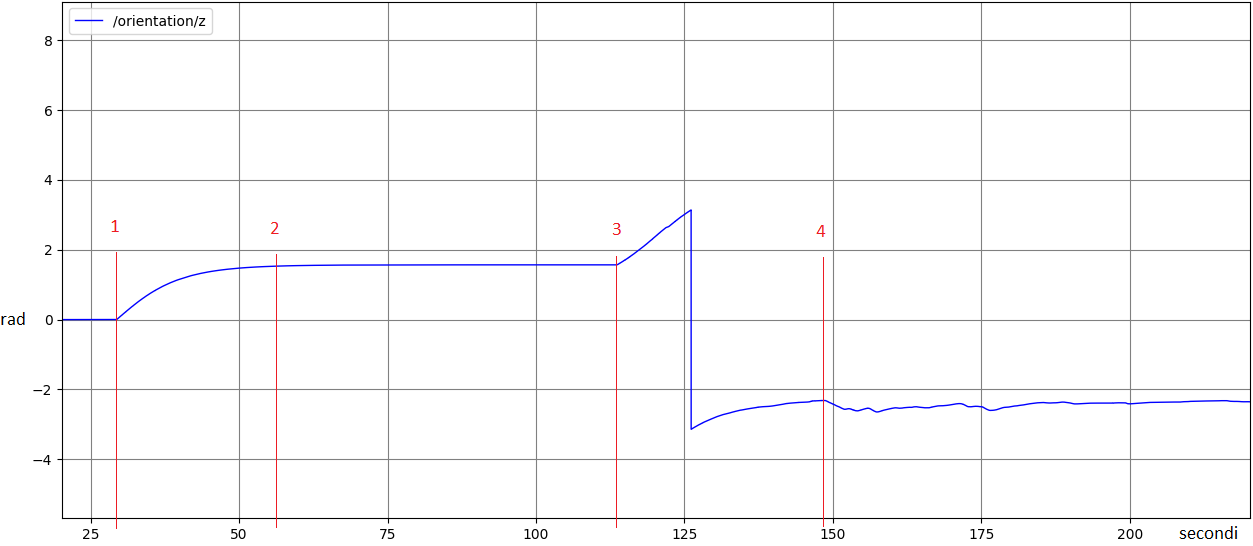
\includegraphics[width=0.9\textwidth]{Appendice2/Figs/segnale_totale_cut.png} } 

\subfloat[Settling iniziale]{
	\label{subfig:settling_iniziale}
	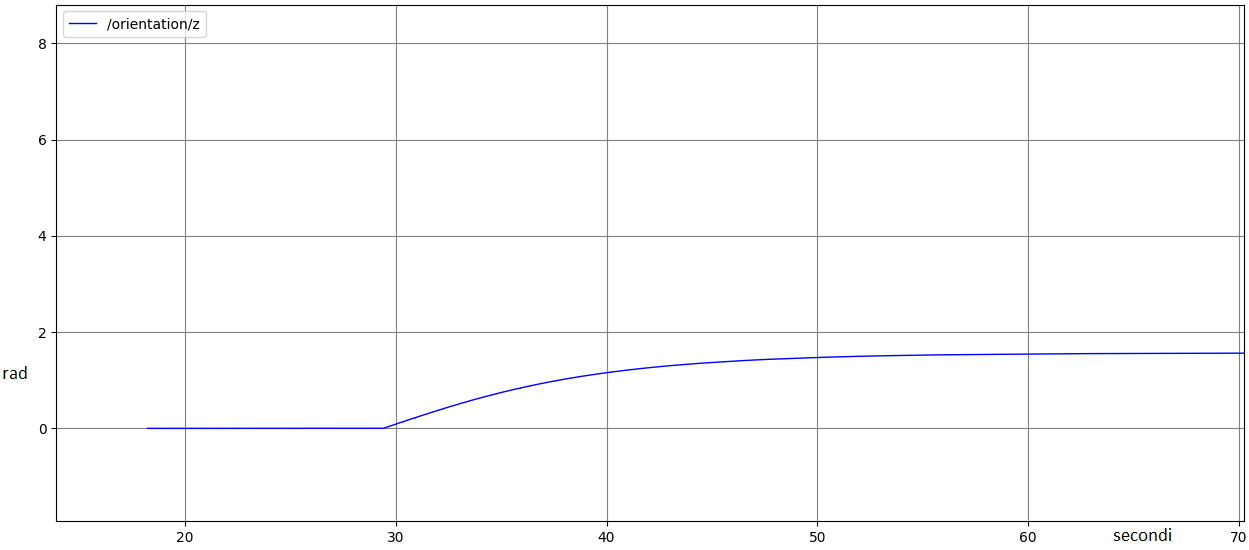
\includegraphics[width=0.9\textwidth]{Appendice2/Figs/settling_iniziale.png} } 

\subfloat[Regime con UWB]{
	\label{subfig:regime_da_uwb}
	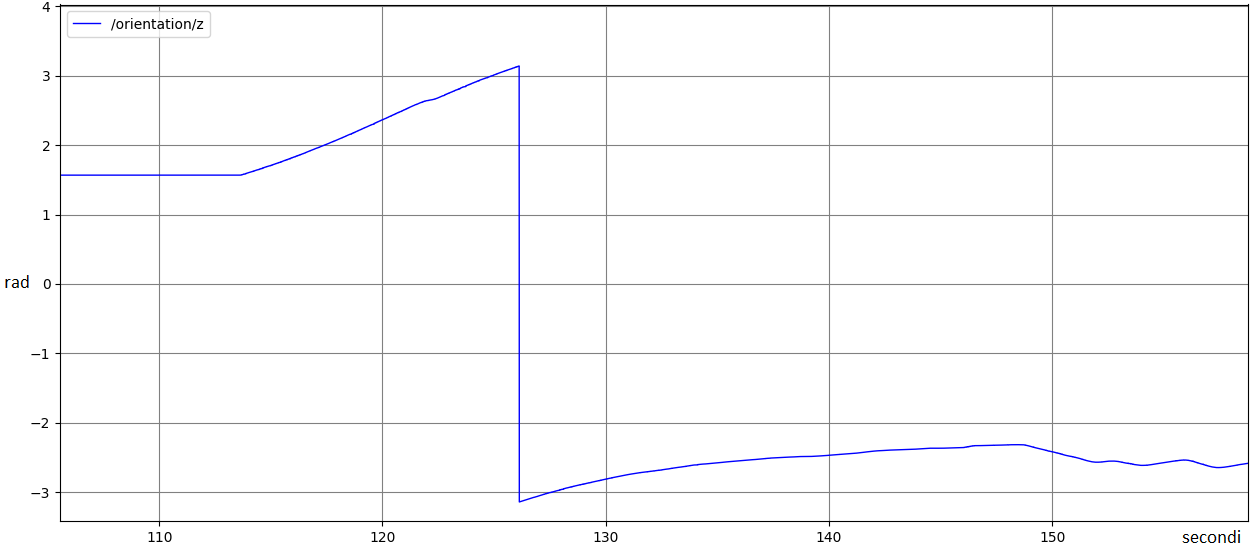
\includegraphics[width=0.9\textwidth]{Appendice2/Figs/regime_da_uwb.png} } 
	
\caption{Grafico dell'analisi del tempo di regime dello yaw letto da STM}
\label{fig:grafico_analisi_yaw}

\end{figure}


%%%%%%%%%%%%%%%%%%%%%%%% FEDE %%%%%%%%%%%%%%%%%%%%%%%%%
Per rimuovere gli outliers si è deciso di basare l'identificazione sullo \texttt{Z-score}. \\
Lo \texttt{Z-score} è una misura che descrive la relazione di un valore rispetto alla media di un gruppo, più precisamente è una misura in termini di deviazione standard dalla media, che può essere positivo se sopra di essa o negativo se al di sotto. 
I dati con valori di \texttt{Z-score} più alti rispetto ad una determinata soglia saranno considerati come outliers, nella maggior parte dei casi tale soglia è pari a 3.

Per calcolarlo verrà usata la funzione \texttt{"stats.zscore()"} facente parte della libreria \texttt{scipy} 

Per prima cosa si calcola la norma due al quadrato di ogni dato raccolto:

\begin{lstlisting}[language=Python]
 for i in range (len(pose_rec_0)):
     data.append( pose_rec_0[i].pose.position.x**2 +
     pose_rec_0[i].pose.position.y**2 + pose_rec_0[i].pose.position.z**2 )
\end{lstlisting}

\bigskip
\bigskip

Poi si crea un \texttt{DataFrame}, una struttura dati di \texttt{Pandas}\footnote{libreria software per \texttt{Python} utilizzata per manipolazione e analisi dei dati.}, che andrà a contenere le norme appena calcolate ed infine si riempe una colonna di tale struttura con i valori dello \texttt{Z-score} associati ad ogni dato. 
A questo punto si riempie l'array \texttt{indexes} con gli indirizzi dei valori che hanno uno \texttt{Z-score} superiore a 3 e quindi classificati come outliers, che poi verranno sfruttati per sapere quali dati andare a rimuovere.
\begin{lstlisting}[language=Python]
import pandas as pd
from scipy import stats
import numpy as np

z_limit = 3

data=[]
# calcola la norma due al quadrato di ogni dato
 for i in range (len(pose_rec_0)):
     data.append(pose_rec_0[i].pose.position.x**2 +
     pose_rec_0[i].pose.position.y**2 + pose_rec_0[i].pose.position.z**2)

# identifica gli outlier basandoti sulla norma due al quadrato e
# salva il loro indice
df= pd.DataFrame({'data':data})
df['z_score']=stats.zscore(df['data'])
indexes = df.loc[df['z_score'].abs()>=z_limit].index 
	
newdata = np.squeeze(df.data)
plt.plot(newdata)

# rimuovi gli elementi in base agli indici degli outlier
 for i in indexes:
     del pose_rec_0[i]
     del data[i]

newdata = np.squeeze(data)
plt.plot(data)
plt.show()
	
rospy.loginfo('outliers eliminati in tag0: %d',
rcvd_msgs_0-len(pose_rec_0))
\end{lstlisting}

\bigskip
\bigskip

\begin{figure}[h!]
\centering

\subfloat[Aspettando lo yaw]{
	\label{subfig:aspetto_lo_yaw}
    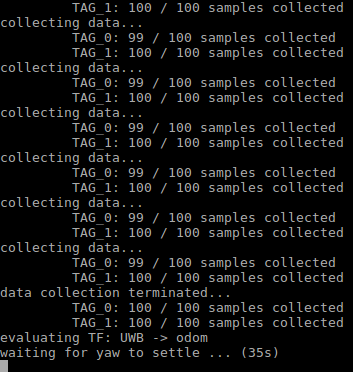
\includegraphics[width=0.5\textwidth]{Appendice2/Figs/aspetto lo yaw.png} } 
\subfloat[Termine procedura]{
	\label{subfig:fine_save_uwb}
	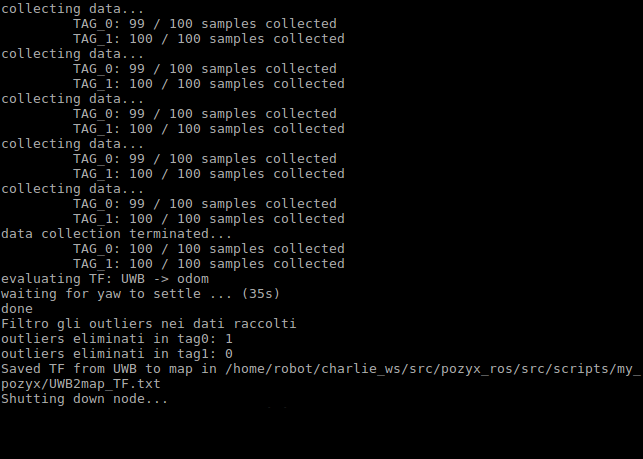
\includegraphics[width=0.5\textwidth]{Appendice2/Figs/fine_save_uwb_map.png} } 
	
\caption{Feedback all'utente dal sistema di salvataggio della posa relativa tra mappa e UWB}
\label{fig:aaaaaaa}

\end{figure}

%%%%%%%%%%%%%%%%%%%%%%%%%%%%%%%%%%%%%%%%%%%%%%%%%%%%%%%

\clearpage

\begin{figure}[ht]
    \centering
    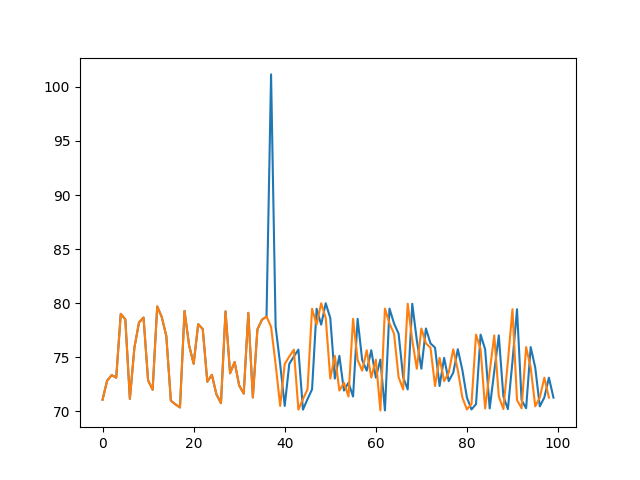
\includegraphics[width=1\textwidth]{Appendice2/Figs/rimozione_outliers.png}
    \caption[Rimozione outlier]{Rimozione outlier}
    \label{fig:rimozione_outlier}
\end{figure}

"\verb!tag_in_map.py!" avvia il nodo che legge dal file \verb!UWB2map_TF.txt! i dati necessari a definire la trasformazione dal frame \verb!UWB! al frame \verb!map!, utilizzati poi per riportare le coordinate delle tag nel frame della mappa. Pubblica quindi la posa del punto medio tra le due tag, con orientazione letta dal topic \verb!/orientation! proveniente dall'STM\textsuperscript\textregistered. Per un riscontro grafico, è possibile osservare i dati convertiti tramite \verb!Rviz! grazie a due \verb!tf! pubblicate da questo nodo (\verb!UWB -> map! e \verb!map -> tag_center_frame!), dove il frame corrispondente al punto medio tra le tag assume il nome di \verb!tag_center_frame!.

\bigskip

"\verb!pose_fix_pub.py!" avvia il nodo che, iscrivendosi ai topic di posa di AMCL e del punto medio tra le tag, controlla che le due non differiscano eccessivamente l'una dall'altra; infatti, può capitare che il sistema di localizzazione Lidar fallisca nel caso in cui l'ambiente sia troppo omogeneo oppure in caso di malfunzionamento del sensore (casuale o indotto). In questa eventualità, la probabilità che il sistema converga nuovamente alla posa corretta senza ausili esterni è molto bassa, per ovviare a ciò si è deciso di sfruttare l'informazione fornita dal sistema UWB che è sempre disponibile e non è soggetta a tali problematiche. Qualora le due pose differiscano più di $1.5$m viene automaticamente pubblicato un fix di posa sul topic \verb!/initialpose! al quale segue una modifica temporanea dei parametri di AMCL in modo da forzare la convergenza del filtro senza necessità del movimento del robot. È stato predisposto un meccanismo di protezione che ferma i motori durante la procedura di correzione e che, una volta terminata, ripristina lo stato precedente del controllo. Questo sistema è stato implementato per evitare movimenti del robot mentre la posizione non è nota (questa funzionalità è attualmente disabilitata). Per una descrizione in dettaglio vedere paragrafo~\ref{localizzazione_robusta}.

\bigskip

"\verb!pose_to_odom.py!" avvia il nodo capace di calcolare l'odometria del robot a partire dai dati di una singola tag. Questi sono pubblicati sia come \texttt{tf} che come topic. 

A causa dei risultati non soddisfacenti ottenuti sfruttando questa sorgente di odometria, si sconsiglia l'utilizzo di questo nodo.

\bigskip

"\texttt{amcl2robot\_pose}" nodo che converte un messaggio di tipo \texttt{PoseWithCovariance-} \texttt{Stamped} fornito da AMCL in un messaggio di tipo \texttt{Point} e lo pubblica sul topic \texttt{/robot\_pose}.

Effettua inoltre un controllo sul funzionamento del sensore Lidar, infatti quando esso è oscurato o non funziona, il campo \verb!intensities! del messaggio LaserScan è riempito con zeri. Se ciò accade la fonte di dati per \texttt{/robot\_pose} diventa il punto medio delle tag\footnote{in coordinate MAP.} e viene mostrato a schermo che è in corso una navigazione basata su UWB.


% ***************************** rplidar\_ros  ***************************** 
\section*{\texttt{rplidar\_ros}}

\begin{itemize}
    \item \verb!rplidarNode!
\end{itemize}

Avvia il sensore Lidar.

% ***************************** laser\_scan\_matcher  *****************************
\section*{\texttt{hector\_slam/hector\_mapping}}
\begin{itemize}
    \item \verb!hector_mapping_node!
\end{itemize}
Nodo standard di \texttt{hector\_mapping} che si occupa di salvare i dati provenienti del Lidar in una mappa.


% ***************************** laser\_scan\_matcher  *****************************
\section*{\texttt{scan\_tools \- kinetic}}
\begin{itemize}
    \item \verb!laser_scan_matcher_node!
\end{itemize}
Nonostante il nome possa trarre in inganno, questo pacchetto non effettua alcun tipo di scan-match con mappa, bensì confronta scan consecutivi (messaggi di tipo \verb!sensor_msgs/LaserScan!) da cui ricava una stima della posizione del laser che pubblica come \verb!geometry_msgs/Pose2D! oppure come \verb!tf!. 
Il pacchetto può essere usato senza stime di odometria provenienti da altri sensori, in questo caso è in grado di fornirne lui stesso una stima; questo è il contesto in cui è attualmente utilizzato il nodo.
Tuttavia nel caso si disponesse di più fonti di odometria, esse possono essere sfruttate per migliorare i risultati.


% ***************************** charlie pkg  *****************************
\section*{\texttt{charlie\_pkg}}
\begin{itemize}
    \item \verb!localization.launch!
\end{itemize}

"\verb!localization.launch!" è il launch file principale del sistema di localizzazione: in primis avvia il Lidar\footnote{I parametri sono standard, volendo si può modificare quello riguardante la porta seriale su cui si trova il Lidar (nel nostro caso \texttt{/ttyUSB0})}, carica la mappa e definisce la trasformazione statica da \verb!base_link! a \verb!laser! (il frame solidale al Lidar) posizionandoli come coincidenti. A questo punto l'ambiente di base per la localizzazione è pronto, si avvia quindi \verb!laser_scan_matcher! (nodo \verb!laser_scan_matcher_node!) che si occupa di fornire l’odometria sotto forma di \verb!tf! necessaria ad AMCL per funzionare; vengono poi avviate le due sorgenti di posa del robot, AMCL, che effettua una stima con il sensore laser, e \verb!tag_in_map!, che porta le componenti di posa del punto medio tra le tag in coordinate nel frame \verb!map!. Si hanno a questo punto le due pose del robot riferite allo stesso frame ed è quindi possibile avviare il sistema di fix di posa lanciando il nodo \verb!pose_fix_pub.py!. Da qui, il sistema di localizzazione robusta è in esecuzione e sono quindi disponibili i dati per guidare del veicolo; vengono quindi avviati il nodo gestore della comunicazione seriale ("\verb!SerialManager!") ed i nodi di interfaccia \verb!amcl2robot_pose! e \verb!navgoal! che predispongono la posa stimata da AMCL ed il goal dato tramite \verb!Rviz! nel formato previsto per l'invio in seriale. Il primo si occupa di convertire la posa di tipo \verb!PoseWithCovarianceStamped! fornita da AMCL in Point dove $x$ ed $y$ sono le coordinate di posizione del robot nella mappa, mentre $z$ rappresenta lo $yaw$, questo è necessario per come è stato progettato il sistema di comunicazione via seriale. Il secondo si occupa di effettuare la stessa operazione appena descritta, sul goal dato a livello grafico su \verb!Rviz!, cosicchè possa essere inviato via seriale.
Per funzionare correttamente deve essere lanciato dopo, o in concomitanza con \verb!start_uwb.launch! per avere accesso ai dati delle UWB.

% ***************************** navigation  ***************************** 
\section*{\texttt{Navigation}}

\begin{itemize}
    \item \verb!DFL.launch! (per usare le tag come odometria)
\end{itemize}

"\verb!DFL.launch!" è un launch file gemello di \verb!localization.launch! che, a differenza di quest'ultimo, non utilizza l'odometria ricavata dal laser, bensì la ottiene dal sistema \verb!UWB!. Dati gli scarsi risultati, questo approccio è stato abbandonato e pertanto non è stata aggiunta alcuna procedura di fix di posa.

% ***************************** SerialManager  ***************************** 
\section*{\texttt{SerialManager}}

\begin{itemize}
    \item \verb!SerialManager!
\end{itemize}

"\verb!SerialManager!" è il nodo che gestisce la comunicazione via seriale, sia in scrittura che lettura.  Sfrutta la porta \verb!/dev/ttyUSB1! con BAUD di $115200$. 

Si iscrive ai topic di posa delle tag e di AMCL\footnote{il topic esatto è \texttt{\/robot\_pose}, che contiene le informazioni di $x$, $y$, $yaw$ prese dalla posa stimata da AMCL}, a \verb!/waypoint_publisher! (su cui sono pubblicati $x$, $y$, $yaw$  della posa desiderata) e \verb!/start_and_stop!(su cui viene pubblicato $0$ o $1$ per disabilitare o abilitare i motori). 

Il codice è abbastanza semplice, si ha una sequenza predefinita di elementi da inviare dove ogni dato viene suddiviso in pacchetti da $4$ byte ed inserito nella posizione corretta; una volta costruita la stringa da inviare, questa viene spedita. In ricezione si legge un solo dato \verb!orientation!, proveniente dall’STM\textsuperscript\textregistered\hspace{1mm}e rappresentante l’heading del veicolo, questo, una volta letto, viene pubblicato sul topic \verb!/orientation!. Per ulteriori dettagli vedere il paragrafo \ref{comunicazione_seriale}.

